% Project - Technical Documentation
%
% Data Acquisition Technologies and Sensor Networks
% Jacobs University Bremen
% Supervisor: Prof. Dr. Fangning Hu
%
% Created on November 13, 2019
%
% Authors:
%   Ralph Florent <r.florent@jacobs-university.de>
%   Diogo Cosin <d.ayresdeoliveira@jacobs-university.de>
%   Eno Ciraku <e.ciraku@jacobs-university.de>
%
% Main entry for the documentation

% ==============================================================================
% START: Preamble
% ==============================================================================
\documentclass{article}

\usepackage{amsmath}
\usepackage{amssymb}
\usepackage[title]{appendix}
\usepackage{array}
\usepackage[british,UKenglish,USenglish]{babel}
\usepackage[backend=biber,style=numeric,sorting=none]{biblatex}
\usepackage[utf8]{inputenc} % required to load before csquotes
\usepackage{csquotes}
\usepackage[dvipsnames]{xcolor}
\usepackage{graphicx}
\usepackage[inner=3cm,outer=3cm,top=3cm,bottom=3cm]{geometry}
\usepackage{hyperref}
\usepackage{minted}
\usepackage{subcaption}
\usepackage{url}

% Override line interspace default configurations
\renewcommand{\baselinestretch}{1.5}

% Override Table default configurations
\setlength{\tabcolsep}{18pt}
\renewcommand{\arraystretch}{1.5}

% Override hyper reference default configurations
\hypersetup{
    colorlinks = true,
    linkcolor = blue,
    anchorcolor = blue,
    citecolor = blue,
    filecolor = blue,
    urlcolor = blue
}
\urlstyle{same}

\addbibresource{references.bib} % Input references by file
\graphicspath{{images/}} % Set path for image preloading

% set default color and style sheets for the scripts
\usemintedstyle{monokai}

\title{
    {
\includegraphics[scale=0.15]{logo-black.png}} \\
    \vspace{1.4cm}
    {\large \textbf{DATA ACQUISITION TECHNOLOGIES AND SENSOR NETWORKS}} \\
    {\large \textbf{Project Report}} \\
    {\large Smart Outlet: Access and Control Your Power Outlets Remotely}
}

\vspace{1.4cm}
\author{ \textit{By Eno Ciraku, Diogo Cosin, \& Ralph Florent}}
\date{November 13, 2019}

\vspace{1.4cm}
% ==============================================================================
% END: Preamble
% ==============================================================================

% ==============================================================================
% START: Scripts
% ==============================================================================
\begin{document}
\maketitle

% Abstract
% Project - Technical Documentation
%
% Data Acquisition Technologies and Sensor Networks
% Jacobs University Bremen
% Supervisor: Prof. Dr. Fangning Hu
%
% Created on November 13, 2019
%
% Authors:
%   Ralph Florent <r.florent@jacobs-university.de>
%   Diogo Cosin <d.ayresdeoliveira@jacobs-university.de>
%   Eno Ciraku <e.ciraku@jacobs-university.de>
%
% Abstract section of the documentation

% ==============================================================================
% START: Abstract
% ==============================================================================

\begin{abstract}
    \textit{[Here goes the absctract of the documentation...]}
\end{abstract}

% ==============================================================================
% END: Abstract
% ==============================================================================
\newpage

% Introduction
% Project - Technical Documentation
%
% Data Acquisition Technologies and Sensor Networks
% Jacobs University Bremen
% Supervisor: Prof. Dr. Fangning Hu
%
% Created on November 13, 2019
%
% Authors:
%   Ralph Florent <r.florent@jacobs-university.de>
%   Diogo Cosin <d.ayresdeoliveira@jacobs-university.de>
%   Eno Ciraku <e.ciraku@jacobs-university.de>
%
% Introductory part of the documentation

% ==============================================================================
% START: Intro
% ==============================================================================

\section{Introduction}

In this report, the solution, specification, and outcomes of the project of a
Smart Outlet is presented as part of the course \textit{Data Acquisition
Technologies and Sensor Networks} grading criteria. The course proposes to
design a wireless sensor network communicating via a web interface with a
database. The recorded data should be visualized graphically through a
web interface.

In this section, we describe our proposed solution, its motivation, and comment
on this report organization.

\subsection{Solution Proposal}

The so-called Smart Outlet (SO) is a power outlet remotely controlled via a webpage
interface. The solution offers a switch \textit{on/off}, which can be toggled
through the previously mentioned webpage. The same webpage also provides a
monitoring feature that allows the users to verify the states of the SO
throughout time tabular and graphically.

The components of the macro solution of the project are given follows:

\begin{itemize}
    \item \textbf{Hardware component:} the power outlet, the controller device,
    and the wireless communication interface;
    \item \textbf{Webpage:} web-interface for controlling the SO states;
    \item \textbf{Database:} relational database for storing the states of the SO.
\end{itemize}

Further details of the solution are introduced in Sections
\ref{sec:inst-resour} and \ref{sec:methodology}.

In this project, we decided to constrain the SO range to a Wireless Local Area
Network (WLAN). However, this limitation can be overcome by exposing the SO
solution in a public HTTP interface. This feature may be implemented in a
possible next step of this project (out of scope in this report).

\subsection{Motivation}

Besides being a requirement to the successful completion of the course
\textit{Data Acquisition Technologies and Sensor Networks}, building the SO
offers many advantages to a possible end user. For these reasons, we
decided to implement a prototype for this solution. These advantages are
described as follows:

\begin{itemize}
    \item \textbf{Convenient usability:} the SO can be controlled from any place
    considering that the webpage may be exposed publicly via HTTP requests;
    \item \textbf{Energy saving:} the user can track the SO state and turn it
    off when considering that it has been unnecessarily used;
    \item \textbf{Multiple users:} the solution enables the access of different
    users through different platforms by only requiring a device that can access
    and visualize webpages exposed on the internet. In other words, users with
    computers, smartphones, and tablets can control the SO.
\end{itemize}

\subsection{Note on the Report Structure}

Before the next Sections of the report, technical details, and results are
presented, let us briefly enlighten how this report is structured as follows:

\begin{itemize}
    \item \textbf{Theoretical review:} theoretical and technical details of the
    chosen hardware components are briefly presented;
    \item \textbf{Instrumentation \& resources:} the integration of the hardware
    and software of the SO prototype is detailed;
    \item \textbf{Methodology:} the techniques, strategies, and procedural
    methods used to implement the core functionality of the project are
    presented;
    \item \textbf{Results \& discussions:} results obtained with the SO
    prototype implementation.
\end{itemize}

%  Do not forget to mention here: goals, problem-solution aspects, keywords
%  (glossary)

% ==============================================================================
% END: Intro
% ==============================================================================

% Theory review
% Project - Technical Documentation
%
% Data Acquisition Technologies and Sensor Networks
% Jacobs University Bremen
% Supervisor: Prof. Dr. Fangning Hu
%
% Created on November 13, 2019
%
% Authors:
%   Ralph Florent <r.florent@jacobs-university.de>
%   Diogo Cosin <d.ayresdeoliveira@jacobs-university.de>
%   Eno Ciraku <e.ciraku@jacobs-university.de>
%
% Theory review for the documentation

% ==============================================================================
% START: Theoretical background
% ==============================================================================

\section{State of Art}
\label{sec:state-of-art}
\textit{[Here goes the state of art part of the documentation...]}

% ==============================================================================
% END: Theoretical background
% ==============================================================================

% Main contents
% Project - Technical Documentation
%
% Data Acquisition Technologies and Sensor Networks
% Jacobs University Bremen
% Supervisor: Prof. Dr. Fangning Hu
%
% Created on November 13, 2019
%
% Authors:
%   Ralph Florent <r.florent@jacobs-university.de>
%   Diogo Cosin <d.ayresdeoliveira@jacobs-university.de>
%   Eno Ciraku <e.ciraku@jacobs-university.de>
%
% 1) Introduction
% 2) Theoretical background
% 3) Instrumentation (software and tools)
% 4) Methods (Procedure)
% 5) Results, Discussions
% 6) Conclusion

% ==============================================================================
% START: Main Content
% ==============================================================================

% Hardware and Software Resources
% Project - Technical Documentation
%
% Data Acquisition Technologies and Sensor Networks
% Jacobs University Bremen
% Supervisor: Prof. Dr. Fangning Hu
%
% Created on November 20, 2019
%
% Authors:
%   Ralph Florent <r.florent@jacobs-university.de>
%   Diogo Cosin <d.ayresdeoliveira@jacobs-university.de>
%   Eno Ciraku <e.ciraku@jacobs-university.de>
%
% Intrumentation and Resources of the documentation

% ==============================================================================
% START: Intrumentation & Resources
% ==============================================================================

\section{Intrumentation \& Resources}
Recalling that the SO prototype is the complete integration of a set of hardware and software, we detail in this section more in-depth specifications on them. Below are enlisted the tools used to set up and carry out successfully the current version of the project.

\subsection{Hardware and other materials}
The SO hardware refers to the physical components that add up to the \emph{Webduino} module. Although there are many possible options in choosing different kinds of hardware to build up the circuitry, we opt for the most reasonable\footnote{Building a separate module from scratch requires time and work, plus other tasks to refine a working component.} choice, which is to reuse already-prebuilt modules and integrate them into one. Hence, in Table \ref{table:hardware-and-materials} are listed the items with their corresponding details.
\begin{table}[!ht]
    \begin{center}
        \begin{tabular}{ |l|l|l|l| }
            \hline
            \multicolumn{4}{ |c| }{ \textbf{ Hardware \& Other Materials }} \\
            \hline % Table headers
             & \textbf{Series} & \textbf{Quantity} & \textbf{Cost}  \\ [0.5ex]
            \hline % Table body (row-wise contents)
            \textbf{\textit{Microcontroller Board}} & MEGA 2560 R3 & 1 & \euro{ 14,99 }  \\
            \hline
            \textbf{\textit{4-Channel Relay}} & GE-EL-SM-006 & 1 & \euro{ 6,99 }  \\
            \hline
            \textbf{\textit{Wi-Fi Module}} & ESP8266-01 & 1 & \euro{ 6,99 } \\
            \hline
        \end{tabular}
        \caption{Detailed information on the hardware and materials used for the SO prototype.}
        \label{table:hardware-and-materials}
    \end{center}
\end{table}

Additionally, other useful materials such as:
\begin{itemize}
    \item 12x male-to-male jumper cables (20 cm)
    \item 12x male-to-female jumper cables (20 cm)
    \item 12x female-to-female jumper cables (20 cm)
    \item 1x access point or router (tp-link TL-WR940N)
    \item 2x computing devices or laptop (Lenovo T460p and Macbook Air)
\end{itemize}
remain useful to connect the different components and have them work as one stable module. More technical specifications are given on each one of the materials and devices, including their working conditions, in the section \emph{State of Art}.

% TODO: touch the budget here

\subsection{Tools and software}
Next, we present the set of tools and software that are used at the time of implementing the prototype:
\begin{itemize}
    \item Operating systems (GNU/Linux, Mac OS, and Windows)
    \item Visual Studio Code (lightweight text editor)
    \item Git\footnote{Git is also available as a bash emulation for other platforms for free (e.g., Git Bash for Windows).} (version control)
    \item GitHub (web-based hosting service for Git versioning system)
    \item Jupyter Notebook (workspace for scripting and simulation)
    \item Arduino IDE (development environment for Arduino boards)
\end{itemize}

% TODO: list current versions in table

Regarding the software versions, it is highly recommended to use the exact versions mentioned in Table 2 to avoid conflicts and compiling errors. On the other hand, the developer can always dig into the breaking changes (if that is the case) that might requires to refactor part of the implementation to have a fully working prototype. However, it is recommended to check the changelog of the updates/releases, if any.

\noindent
Note that some tools mentioned above are just a matter of personal preferences. Other preferred options are more than welcome as long as the developer keeps in mind development speed and productivity. For example, many developers would choose \href{https://www.sublimetext.com/}{Sublime} over \emph{Visual Studio Code}. But they both end up facilitating the same routine: text edition.

\subsection{Programming languages}
Finally, we use the following programming languages:
\begin{itemize}
    \item C/C++ (for the webduino)
    \item Python (for the web API service)
    \item Angular Framework - JavaScript/TypeScript (for the web application)
\end{itemize}

\noindent
\textbf{Important}: \textit{Though we highly recommend that the exact versions of the software and the exact series/models of the materials/devices are used to test out or replicate this project, keep in mind that these hardware might no longer be available in the market as well as the software components might be outdated at some point in time. If that is the case, stay alerted to the updates as we intend to support this project until 2022.}

% ==============================================================================
% END: Intrumentation & Resources
% ==============================================================================

% Methodology
% Project - Technical Documentation
%
% Data Acquisition Technologies and Sensor Networks
% Jacobs University Bremen
% Supervisor: Prof. Dr. Fangning Hu
%
% Created on November 20, 2019
%
% Authors:
%   Ralph Florent <r.florent@jacobs-university.de>
%   Diogo Cosin <d.ayresdeoliveira@jacobs-university.de>
%   Eno Ciraku <e.ciraku@jacobs-university.de>

% ==============================================================================
% START: Methodology
% ==============================================================================

\section{Methodology}
\label{sec:methodology}
In this section, we describe the techniques and strategies, as well as the procedural methods used to implement the core functionality of this project. This description includes the components of the system, the workflow diagram, the third-party libraries, the algorithm and data structure, and finally, the code implementation.

It is essential to stand out the fact that we use external resources to come up
with daily results in terms of programming tools and full-on working devices.
That is, before adventuring into using the materials and devices as well as the appropriate software tools, different research sources were consulted. Some of
these resources are the datasheets of both the prebuilt modules and the
materials, the assistance of the instructor and teaching assistants (TAs),
search engines (mainly Google Search/Internet), and, finally, some related books
and references (e.g. materials provided by the professor).

Being exceptionally helpful, these resources have been the source of truth for any decision-making regarding the correct use of the hardware modules.

\subsection{Components of the prototype}
Roughly speaking, Smart Outlet comprises 3 (three) principal modules:
\begin{itemize}
    \item \textbf{Webduino:} a low-level, modular circuitry formed by an Arduino and a network of sensors. The Arduino board, a microcontroller, acts as a supervisor of microtasks. Being the core component of the hardware systems, it controls the different input/output functions of the connected chips.
    \item \textbf{Web API:} an API service attending HTTP requests from the \emph{webduino} (its only consumer). It coordinates the communication between the Wi-Fi module of the webduino (client) over the air medium (wireless) and the available API resources on an HTTP server. The API service contains various layers of interactions, including the database for data persistence.
    \item \textbf{Web APP:} (short for web application) a single page application (SPA) to visualize the historical content or executed actions during the webduino's operations. It allows user-friendly interactions between an end-user and the prototype itself. The web app is also responsive. That is, it can be accessed and used via mobile devices (tablets, smartphones, etc.).
\end{itemize}

Each one of these modules deep down contains a set of characteristics that
requires more than a brief description to highlight their corresponding
functionality. However, in this document, we intend to explain only how to connect
them and make them work properly as a whole. We indeed provide full
access to the online repository as specified in Appendix \ref{sec:code-repo} so
that anyone can dig any further into the datasheets if needs be.

\subsection{Workflow diagram}
The Smart Outlet project has an easy-to-understand workflow. This workflow explains how each module is connected (not fully as in a mesh connection) and performs a specific task. In this case, we provide a diagram and explain the corresponding role of the inner contents taking part in that workflow in other to achieve the complete functionality of Smart Outlet as a whole.

As shown in Figure \ref{fig:workflow-diagram}, the workflow diagram consists of the following parts:
\begin{itemize}
    \item \textbf{Devices accessing the web application:} a user can use smartphones or desktops (laptops) to access and load the web application. This end-user device should be connected to the local area network (LAN) with this IP: \texttt{192.168.0.0/24}.
    \item \textbf{Server infrastructure:}
    \begin{itemize}
        \item an HTTP server to serve the website when the user browses its web
        address\footnote{Note that a web address, in this case, is the associated
        IP address and the port where the Apache 2.0 service is running. (e.g
        192.168.0.105:4200)};
        \item an API service to attend the requests from consumers (webduino and web app).
    \end{itemize}
    \item \textbf{Webduino:} the hardware module or prototype connected to the same network waiting to update the states of the outlets, if any.
    \item \textbf{Router:} working like a switch, assures connectivity and communication between the other components of the system.
\end{itemize}

\textbf{\textit{Important}}: \textit{Although every connected device lands on the same network, it is highly important to understand that no direct connectivity between the web application and the webduino is established. Refer to UML diagram in Figure \ref{fig:uml-diagram} to get a better idea of how this interaction is made. To illustrate this point, if we had architected the diagramming system this way, we would confront serious problems at the time of taking the web service to public. That is, routing to a local IP (when there are some many security concerns to consider) would be troublesome.}

\begin{figure}[ht!]
    \centering
    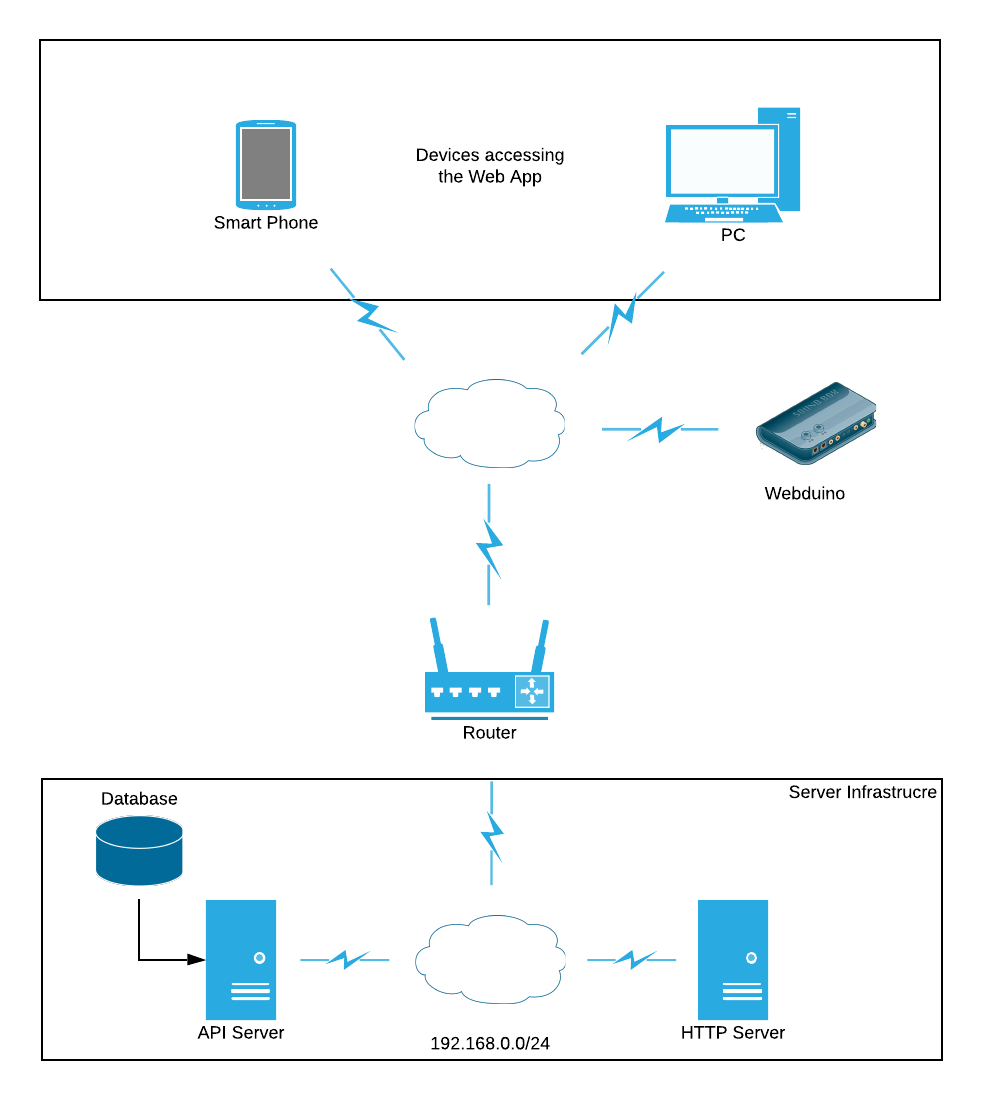
\includegraphics[scale=0.33]{diagrams/workflow.png}
    \caption{Workflow diagram - this is an architecture diagram that displays how every component of the system is interconnected in a real-world situation. (credits: made with \emph{Lucidchart})}
    \label{fig:workflow-diagram}
\end{figure}

\noindent
How do the components interact with each other? Observe the \emph{UML (Unified Modeling Language)} in Figure \ref{fig:uml-diagram} to grasp the idea faster as it is a visual aid to display the sequence of events occurring when the prototype is operating.
\begin{enumerate}
    \item Given the initial conditions, all the components are considered up and running properly;\footnote{The devices (database, API web service, webduino) should be powered on and running. Each device should be assigned a local IP address and should be reachable by other devices over the network.}
    \item A user accessing a web browser may load and view the last updates of the power outlets. When a user updates\footnote{Set an update for a power outlet is basically to change its state from ON-OFF or vice-versa.} the state of an outlet, the changes are saved into the database through the API service and immediately (~2 seconds) reflected in the webduino.
    \item The webduino will constantly attempt to request the last states of the power outlets from the web API service. Once obtained the data, it proceeds by updating the states of the relays, which in turn will open or close the switch of the corresponding power outlet(s).
    \item The historical records can also be visualized on separate views using both a tabular form and a scatter plot.
\end{enumerate}

\begin{figure}[ht!]
    \centering
    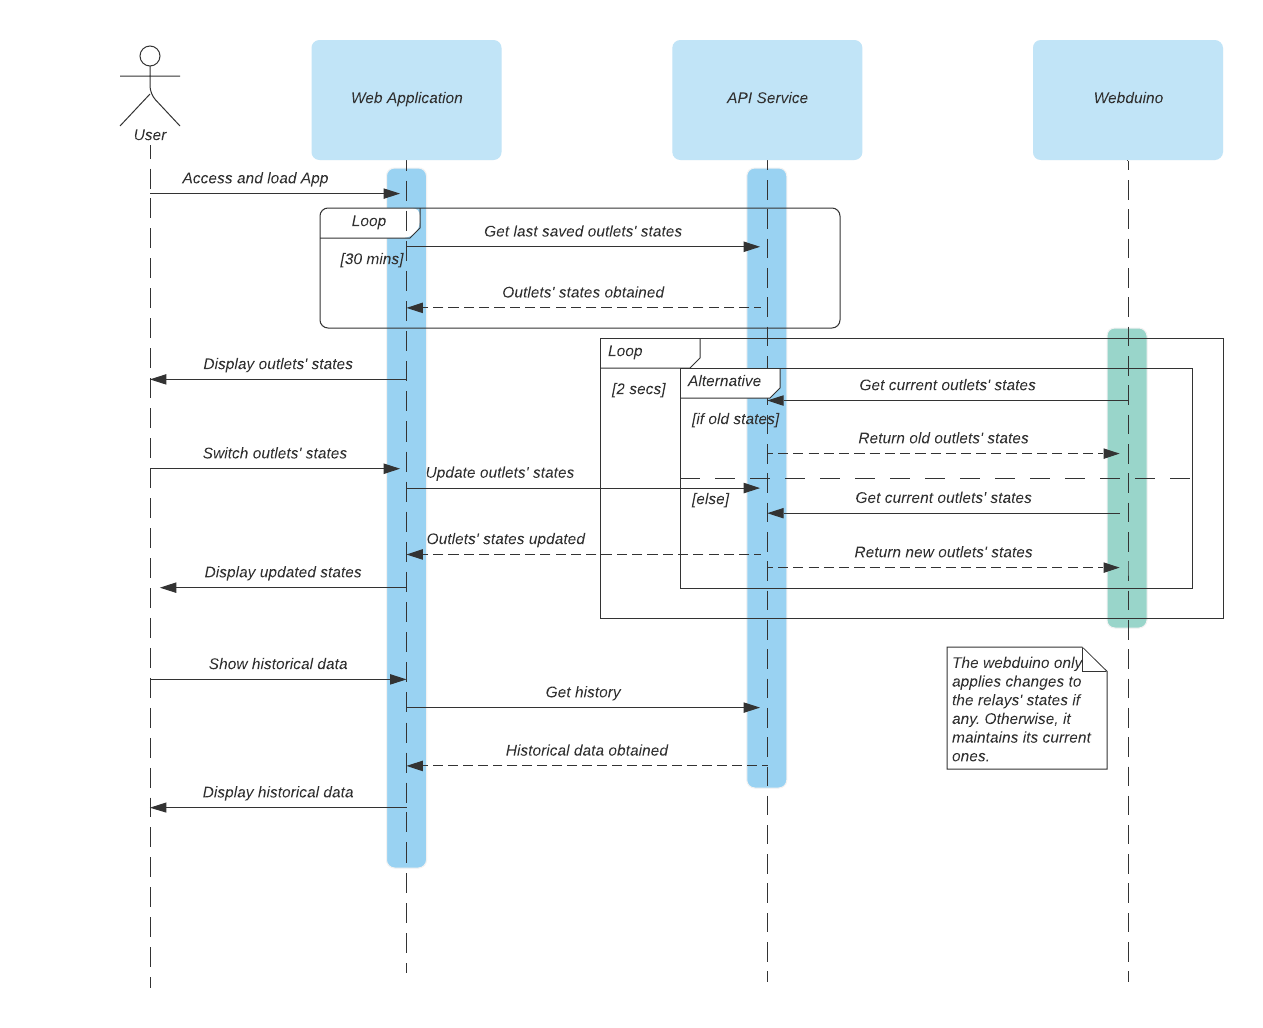
\includegraphics[scale=0.33]{diagrams/uml.png}
    \caption{UML sequence diagram - this shows how every object (web app, API, webduino) within the Smart Outlet system interacts with each other and the order where these interactions take place. (credits: made with \emph{Lucidchart})}
    \label{fig:uml-diagram}
\end{figure}

\subsection{Algorithm and data structure}
Recall that the project touches different development environments. These
environments require different architectures, techniques of programming as well
as the programming languages used. As the line of thinking is distinct for every module, this section discusses each environment separately and eventually shows how
they relate to each other.

\subsubsection{Webduino}
The Smart Outlet prototype, also known as \emph{webduino}, is the final
integrated piece of hardware obtained when combining the microcontroller
(Arduino board), the relay module, and the Wi-Fi (ESP8266-01) module. Since we
are dealing with different kinds of prebuilt submodules, we proceed by evaluating their functionality under a pilot conceptual test. More details on these tests are provided in Section \ref{sec:res-and-disc}.

Arduino supports coding in C/C++ and the concept of Object-Oriented Programming
(OOP). This capability gives us an advantage on how to better organize the code.
After different attempts to optimize the code, we end up using a class-based
structure that facilitates the handling of the relay, that is, the
\textit{ON-OFF} switch, and finally, convert it into a reusable library. Observe
for example in Listing \ref{lst:outlet-class} the class definition representing
an outlet.

\begin{listing}[H]
    \inputminted
    [
        frame=lines,
        framesep=2mm,
        baselinestretch=1.2, % interspace size
        bgcolor=lightgray,
        fontsize=\footnotesize,
        linenos % show line numbers
    ]
    {cpp}{scripts/outlet-class.h}
    \caption{Example of class definition of \textcolor{blue}{Outlet}}
    \label{lst:outlet-class}
\end{listing}

We create and use other utilities as well as helper functions to achieve the final implementation. Similarly, we use this external library  \textit{ArduinoJson} to parse JSON data coming from the server.

The overall logic is quite simple: when the Arduino starts, the submodules' setups are initialized and then fall in an infinite \emph{loop} while executing
an updating status check from the API service. Note the same coded logic in
Listing \ref{lst:outlet-update}. Keep in mind that the entire code is publicly
available and can be consulted for further reading and understanding, as
specified in Appendix \ref{sec:code-repo}.

\begin{listing}[H]
    \inputminted
    [
        frame=lines,
        framesep=2mm,
        baselinestretch=1.2, % interspace size
        bgcolor=lightgray,
        fontsize=\footnotesize,
        linenos % show line numbers
    ]
    {c}{scripts/outlet-update.c}
    \caption{Continuous checks for updating relays' states}
    \label{lst:outlet-update}
\end{listing}

After running the sample tests for every separate module, we put them all together and test them out as one module. And to run the webduino independently, we make the response data available by using a mock API.

\subsubsection{Web API}

The WEB API (abbreviation for Application Programming Interface) provides read
and write access to the states of the relays, stored in the relational
database MySQL. For that, three endpoints are designed with the aid of the
Python micro web framework Flask. Their functions are given as follows:

\begin{itemize}
    \item \textbf{status:} GET interface to provide the status of the outlets in
    JSON format (see Figure \ref{fig:api-status} for the response format);
    \item \textbf{statusino:} GET interface to provide the status of the outlets
    in JSON format in a lighter version. This endpoint is specifically designed
    for the communication with the Arduino to save data transmission.
    This way, the field \textit{updatedOn} is ommited from the response as it is
    not necessary for the correct control of the outlets;
    \item \textbf{update:} POST interface to update the status of the outlets in
    the database;
    \item \textbf{history:} GET interface to provide the historical data for the
    status of the outlets (see Figure \ref{fig:api-history} for the response format).
\end{itemize}

\begin{figure}[h!]
    \centering
    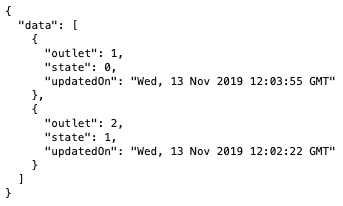
\includegraphics[scale=0.5]{api/status.png}
    \caption{An example of the endpoint \textit{status} response.}
    \label{fig:api-status}
\end{figure}

\begin{figure}[h!]
    \centering
    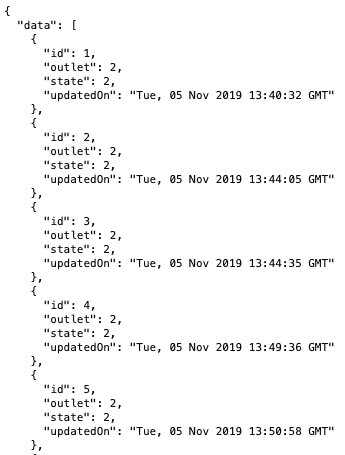
\includegraphics[scale=0.5]{api/history.png}
    \caption{An example of the endpoint \textit{history} response.}
    \label{fig:api-history}
\end{figure}

\subsubsection{Web Application}
The Web App (short for web application), also known as the \emph{Web UI} module
of this project, is an Angular-based\footnote{Consult the README.md markdown
file to learn about the installation and running process when using Angular.}
application. \href{https://angular.io}{Angular} is a JavaScript framework used
for building web applications in a fast yet effective manner. It contains
appealing features and is powered by Google.

As a single web application, the routing done via views. The main components or views of the web app are:
\begin{itemize}
    \item \textbf{home:} a splash screen page serving as the entry point of the web app (see Figure \ref{fig:ui-home}). It also describes the web page purposes;
    \item \textbf{outlets:} a page to perform updates on the outlets' states (See Figure \ref{fig:ui-outlets}). A user can both view and change the states of the currently available outlets;
    \item \textbf{history:} a page to have a basic overview of the past saved
    data in tabular (see Figure \ref{fig:ui-history}) and graph format (see
    Figure \ref{fig:ui-plot}).
\end{itemize}

\begin{figure}[ht!]
    \centering
    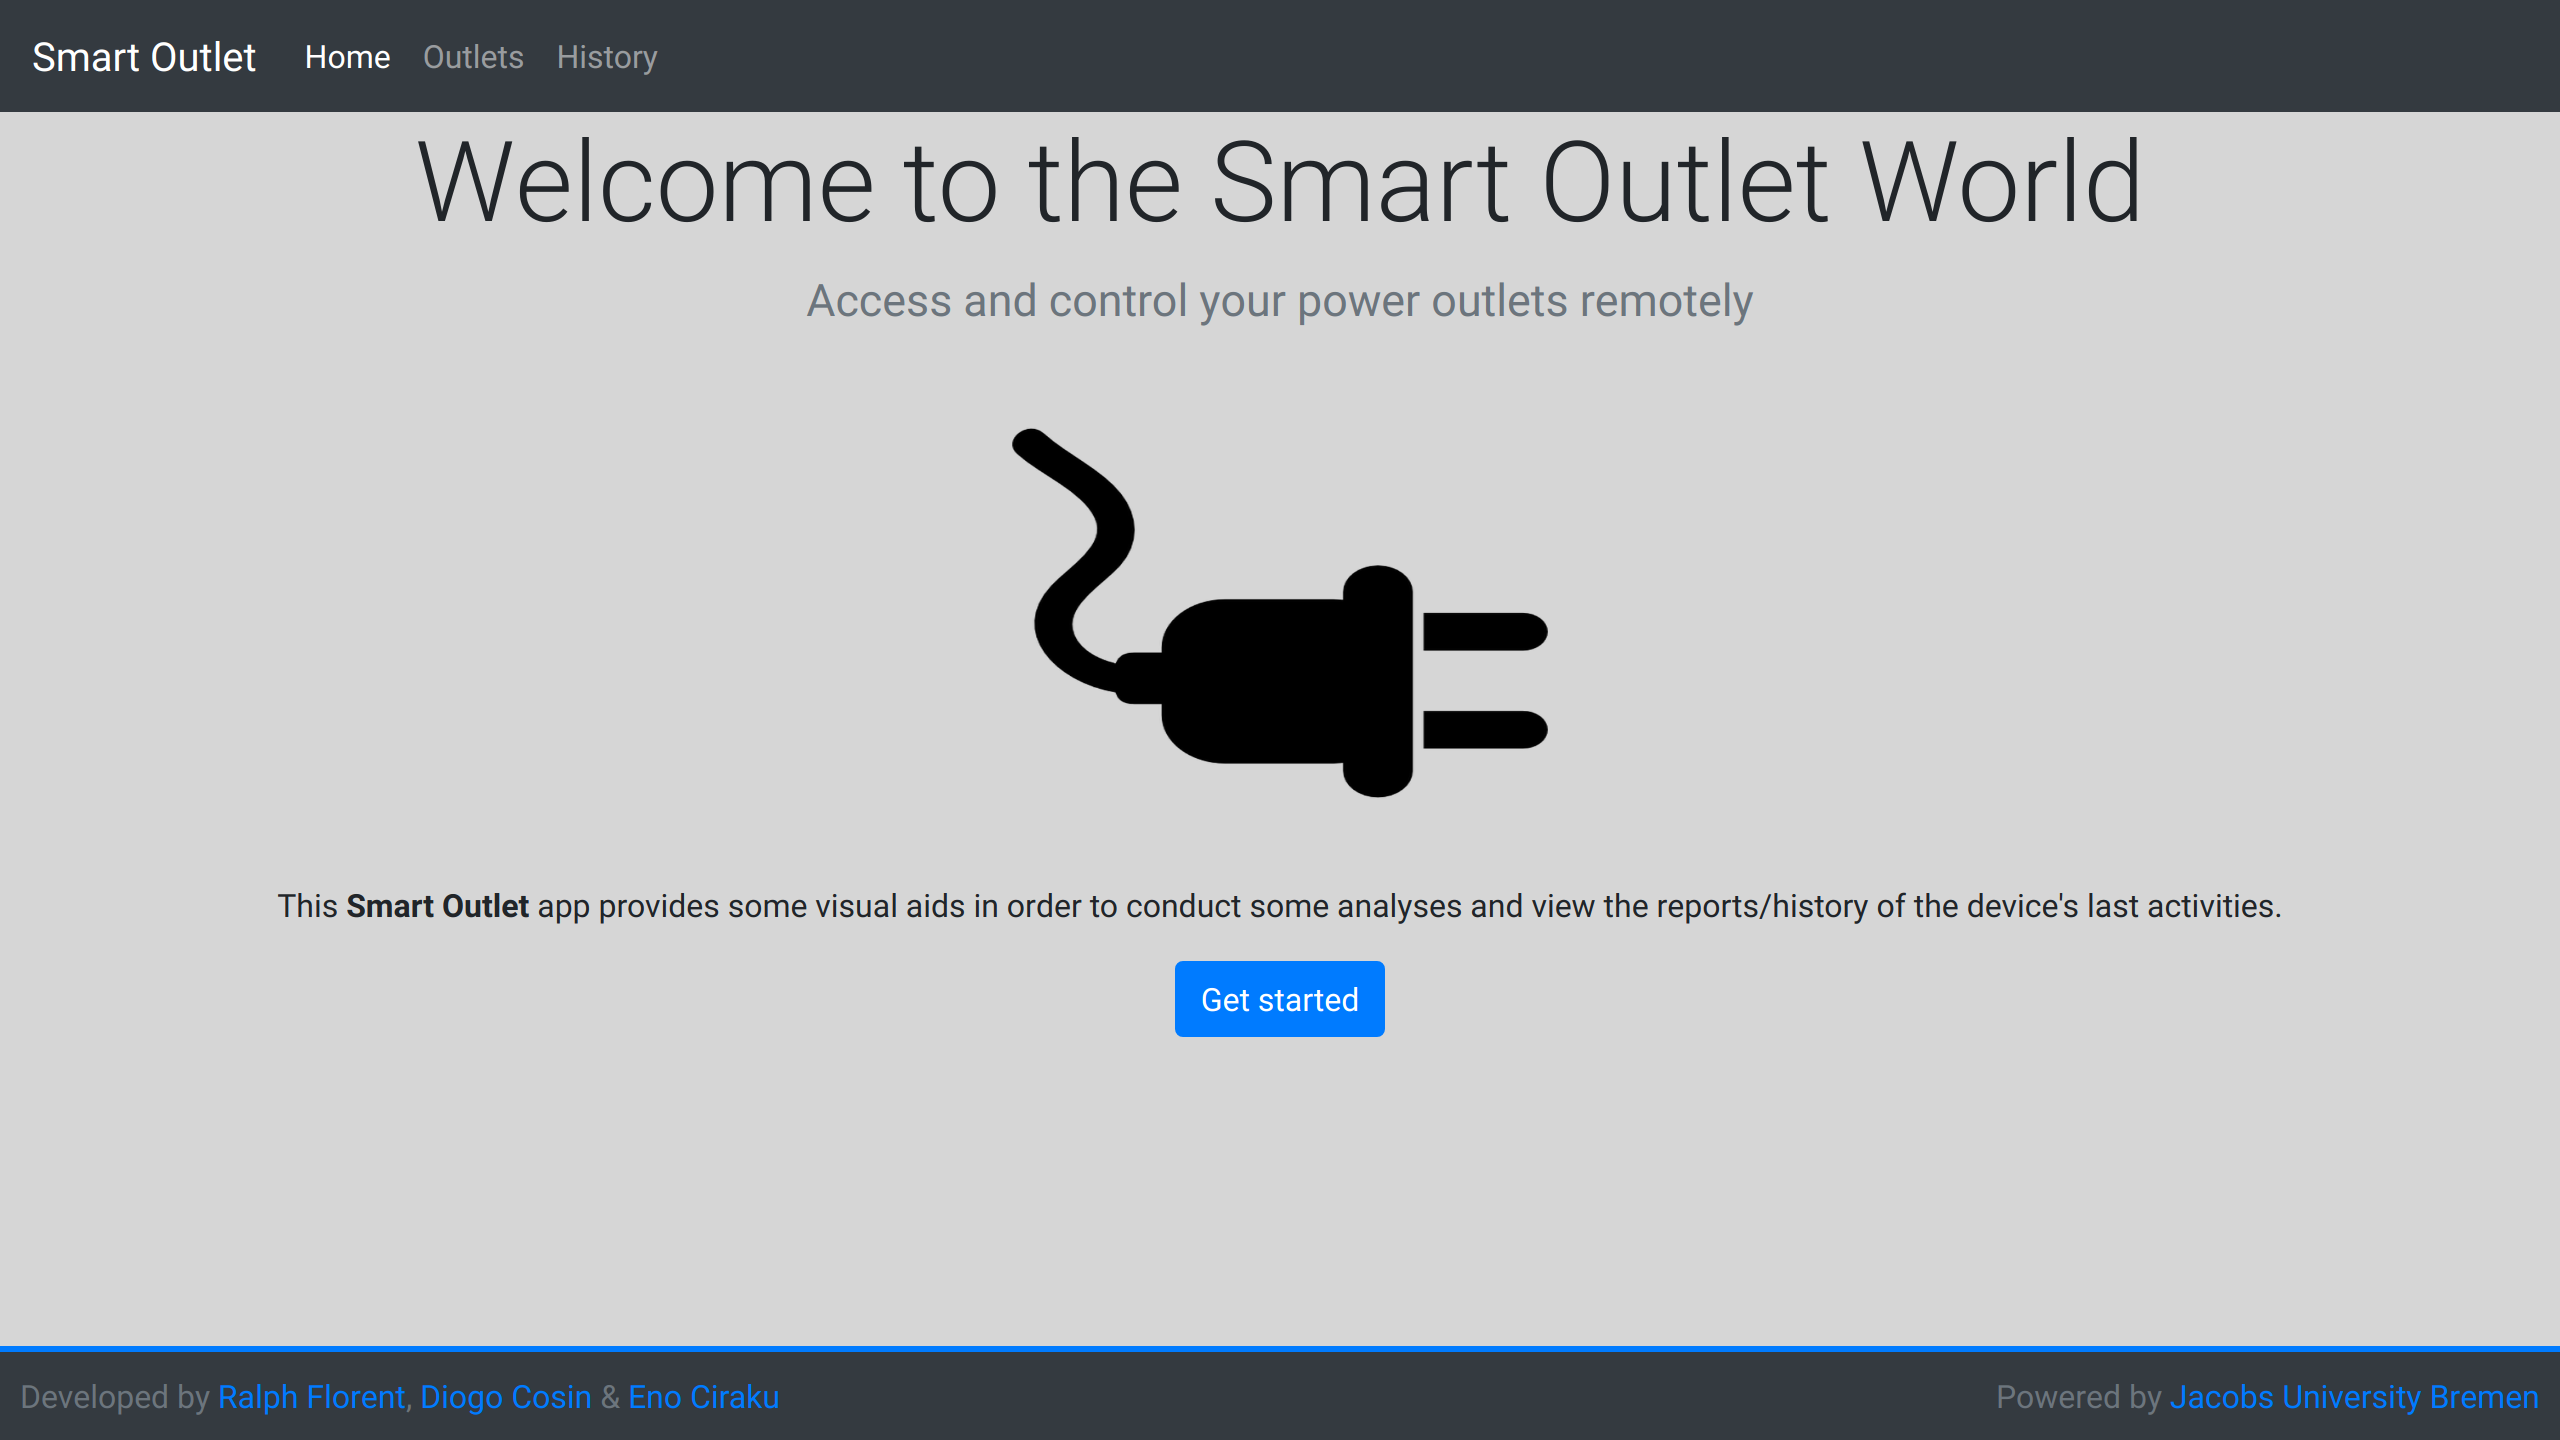
\includegraphics[scale=0.15]{screenshots/web-app/home.png}
    \caption{View of the home page}
    \label{fig:ui-home}
\end{figure}

\begin{figure}[ht!]
    \centering
    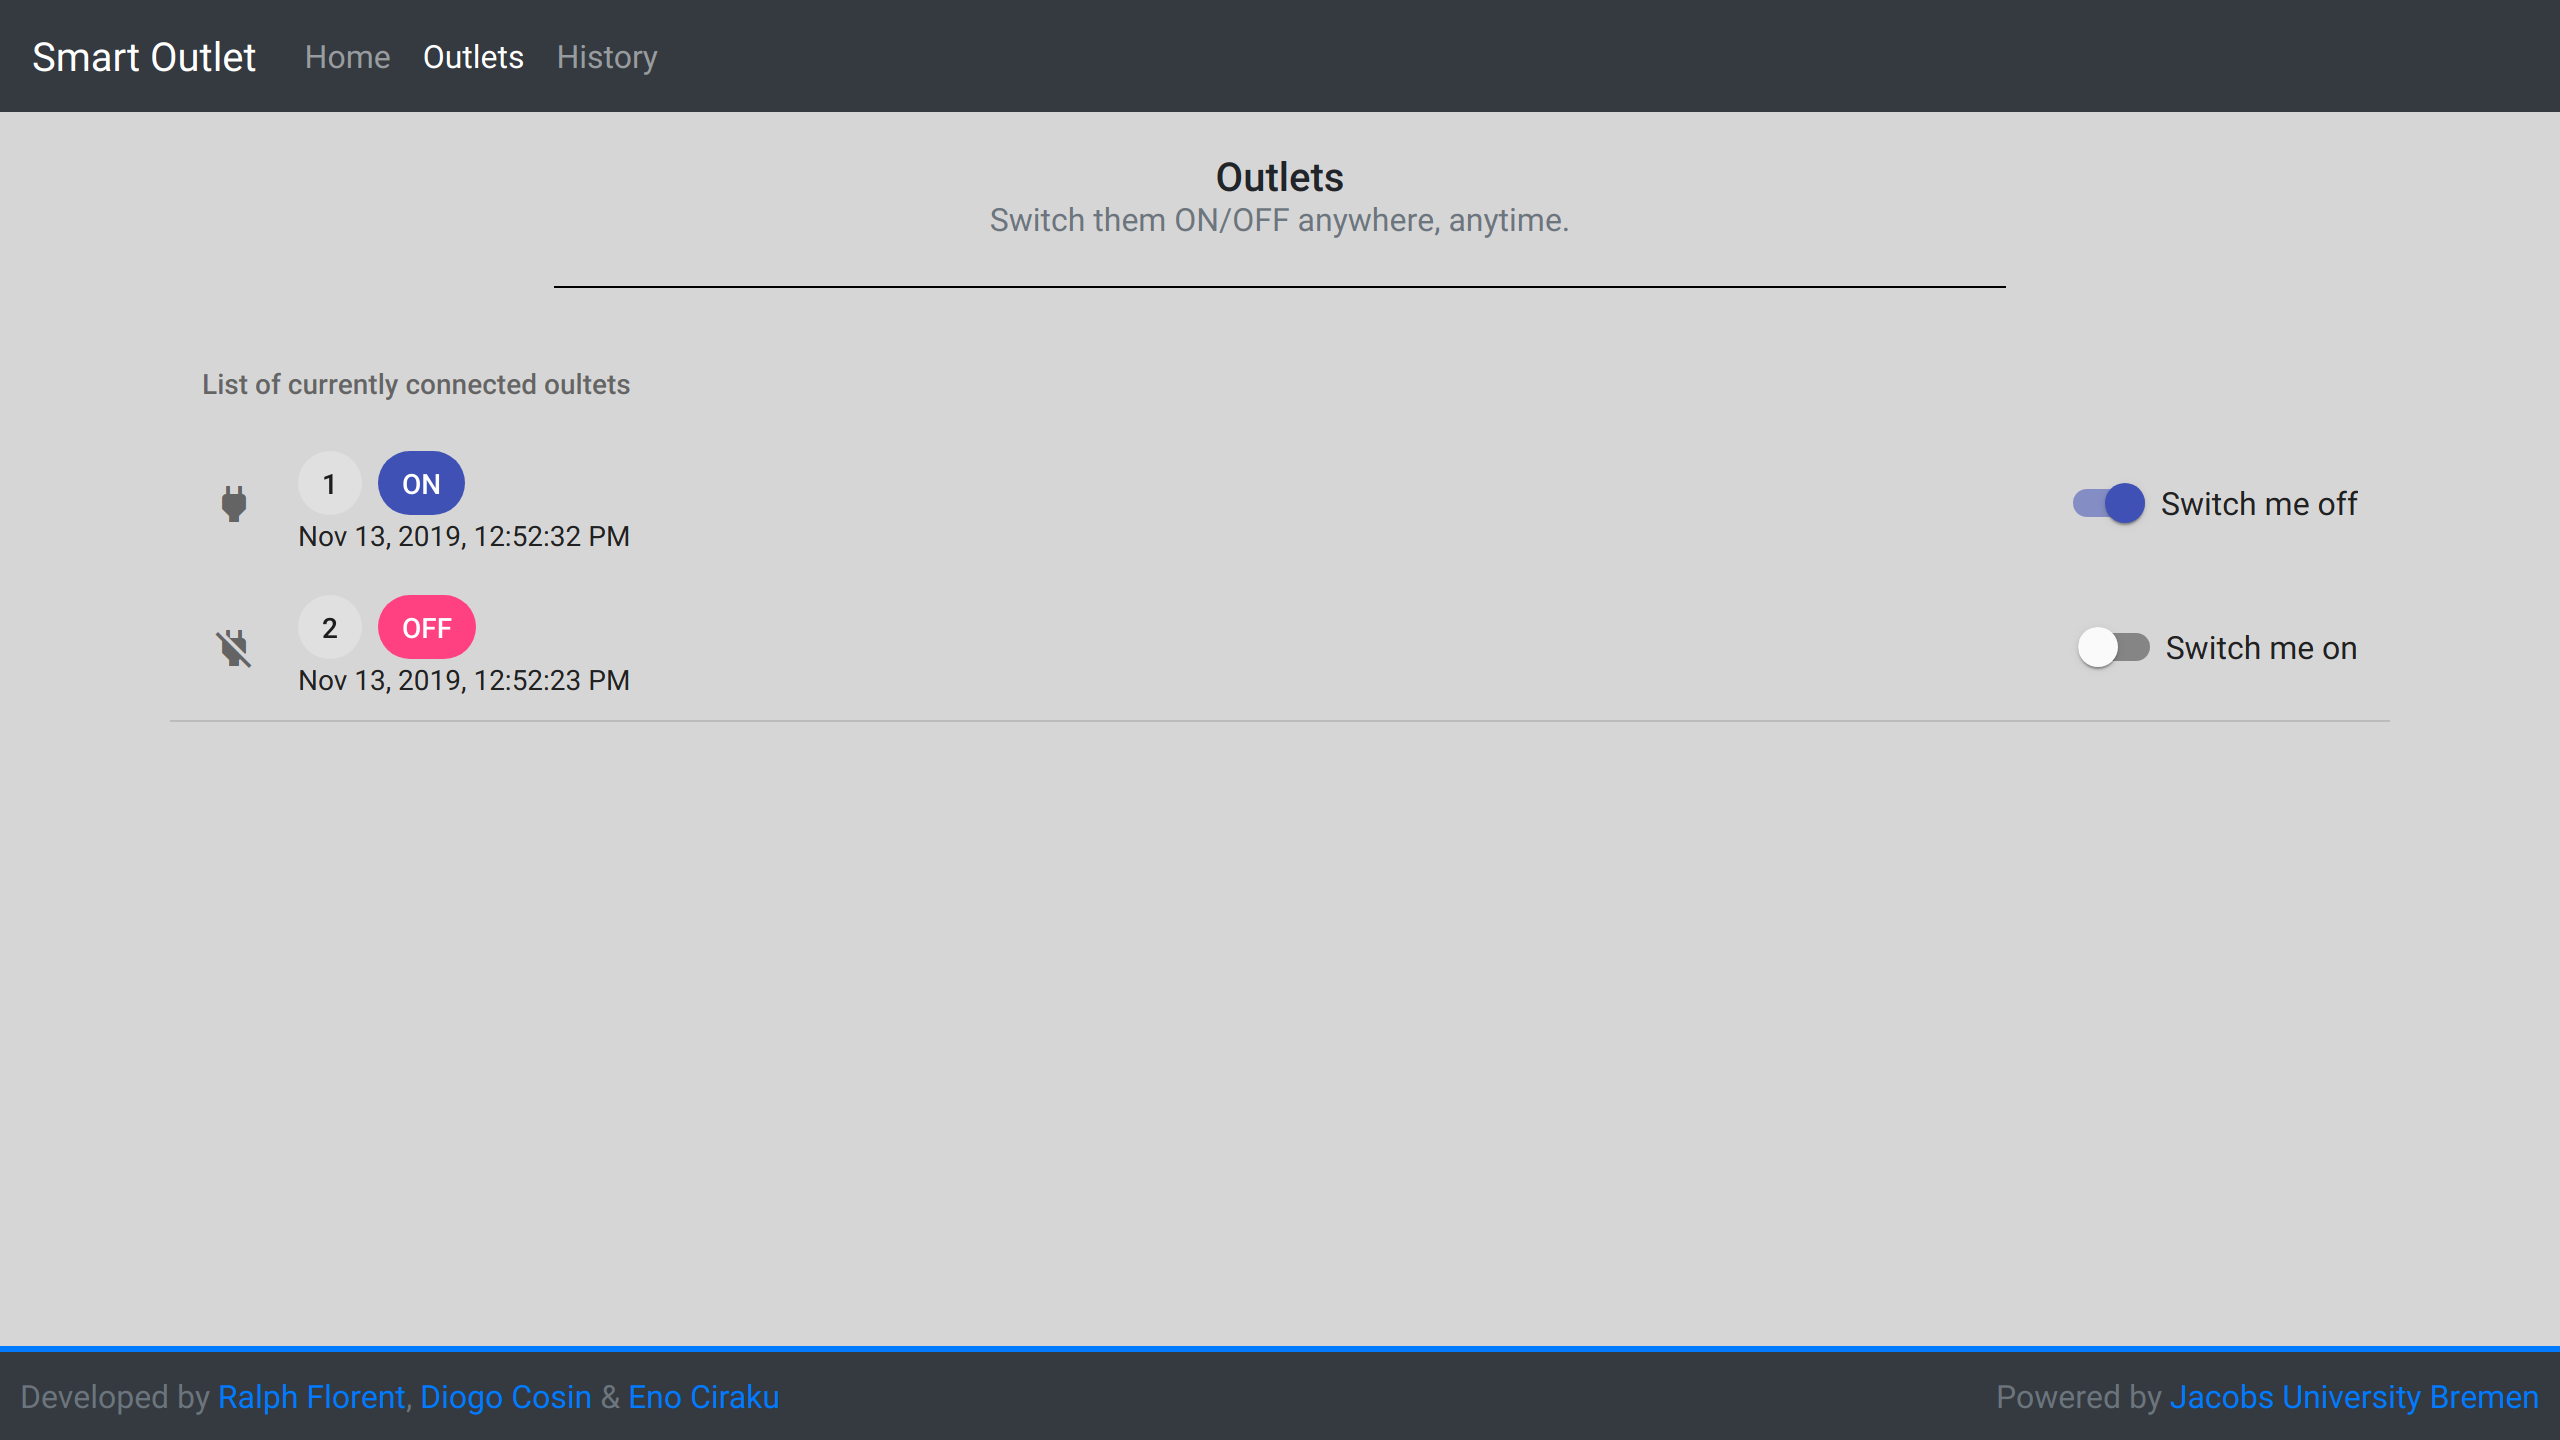
\includegraphics[scale=0.15]{screenshots/web-app/outlets.png}
    \caption{View of the outlets page}
    \label{fig:ui-outlets}
\end{figure}

\begin{figure}[ht!]
    \centering
    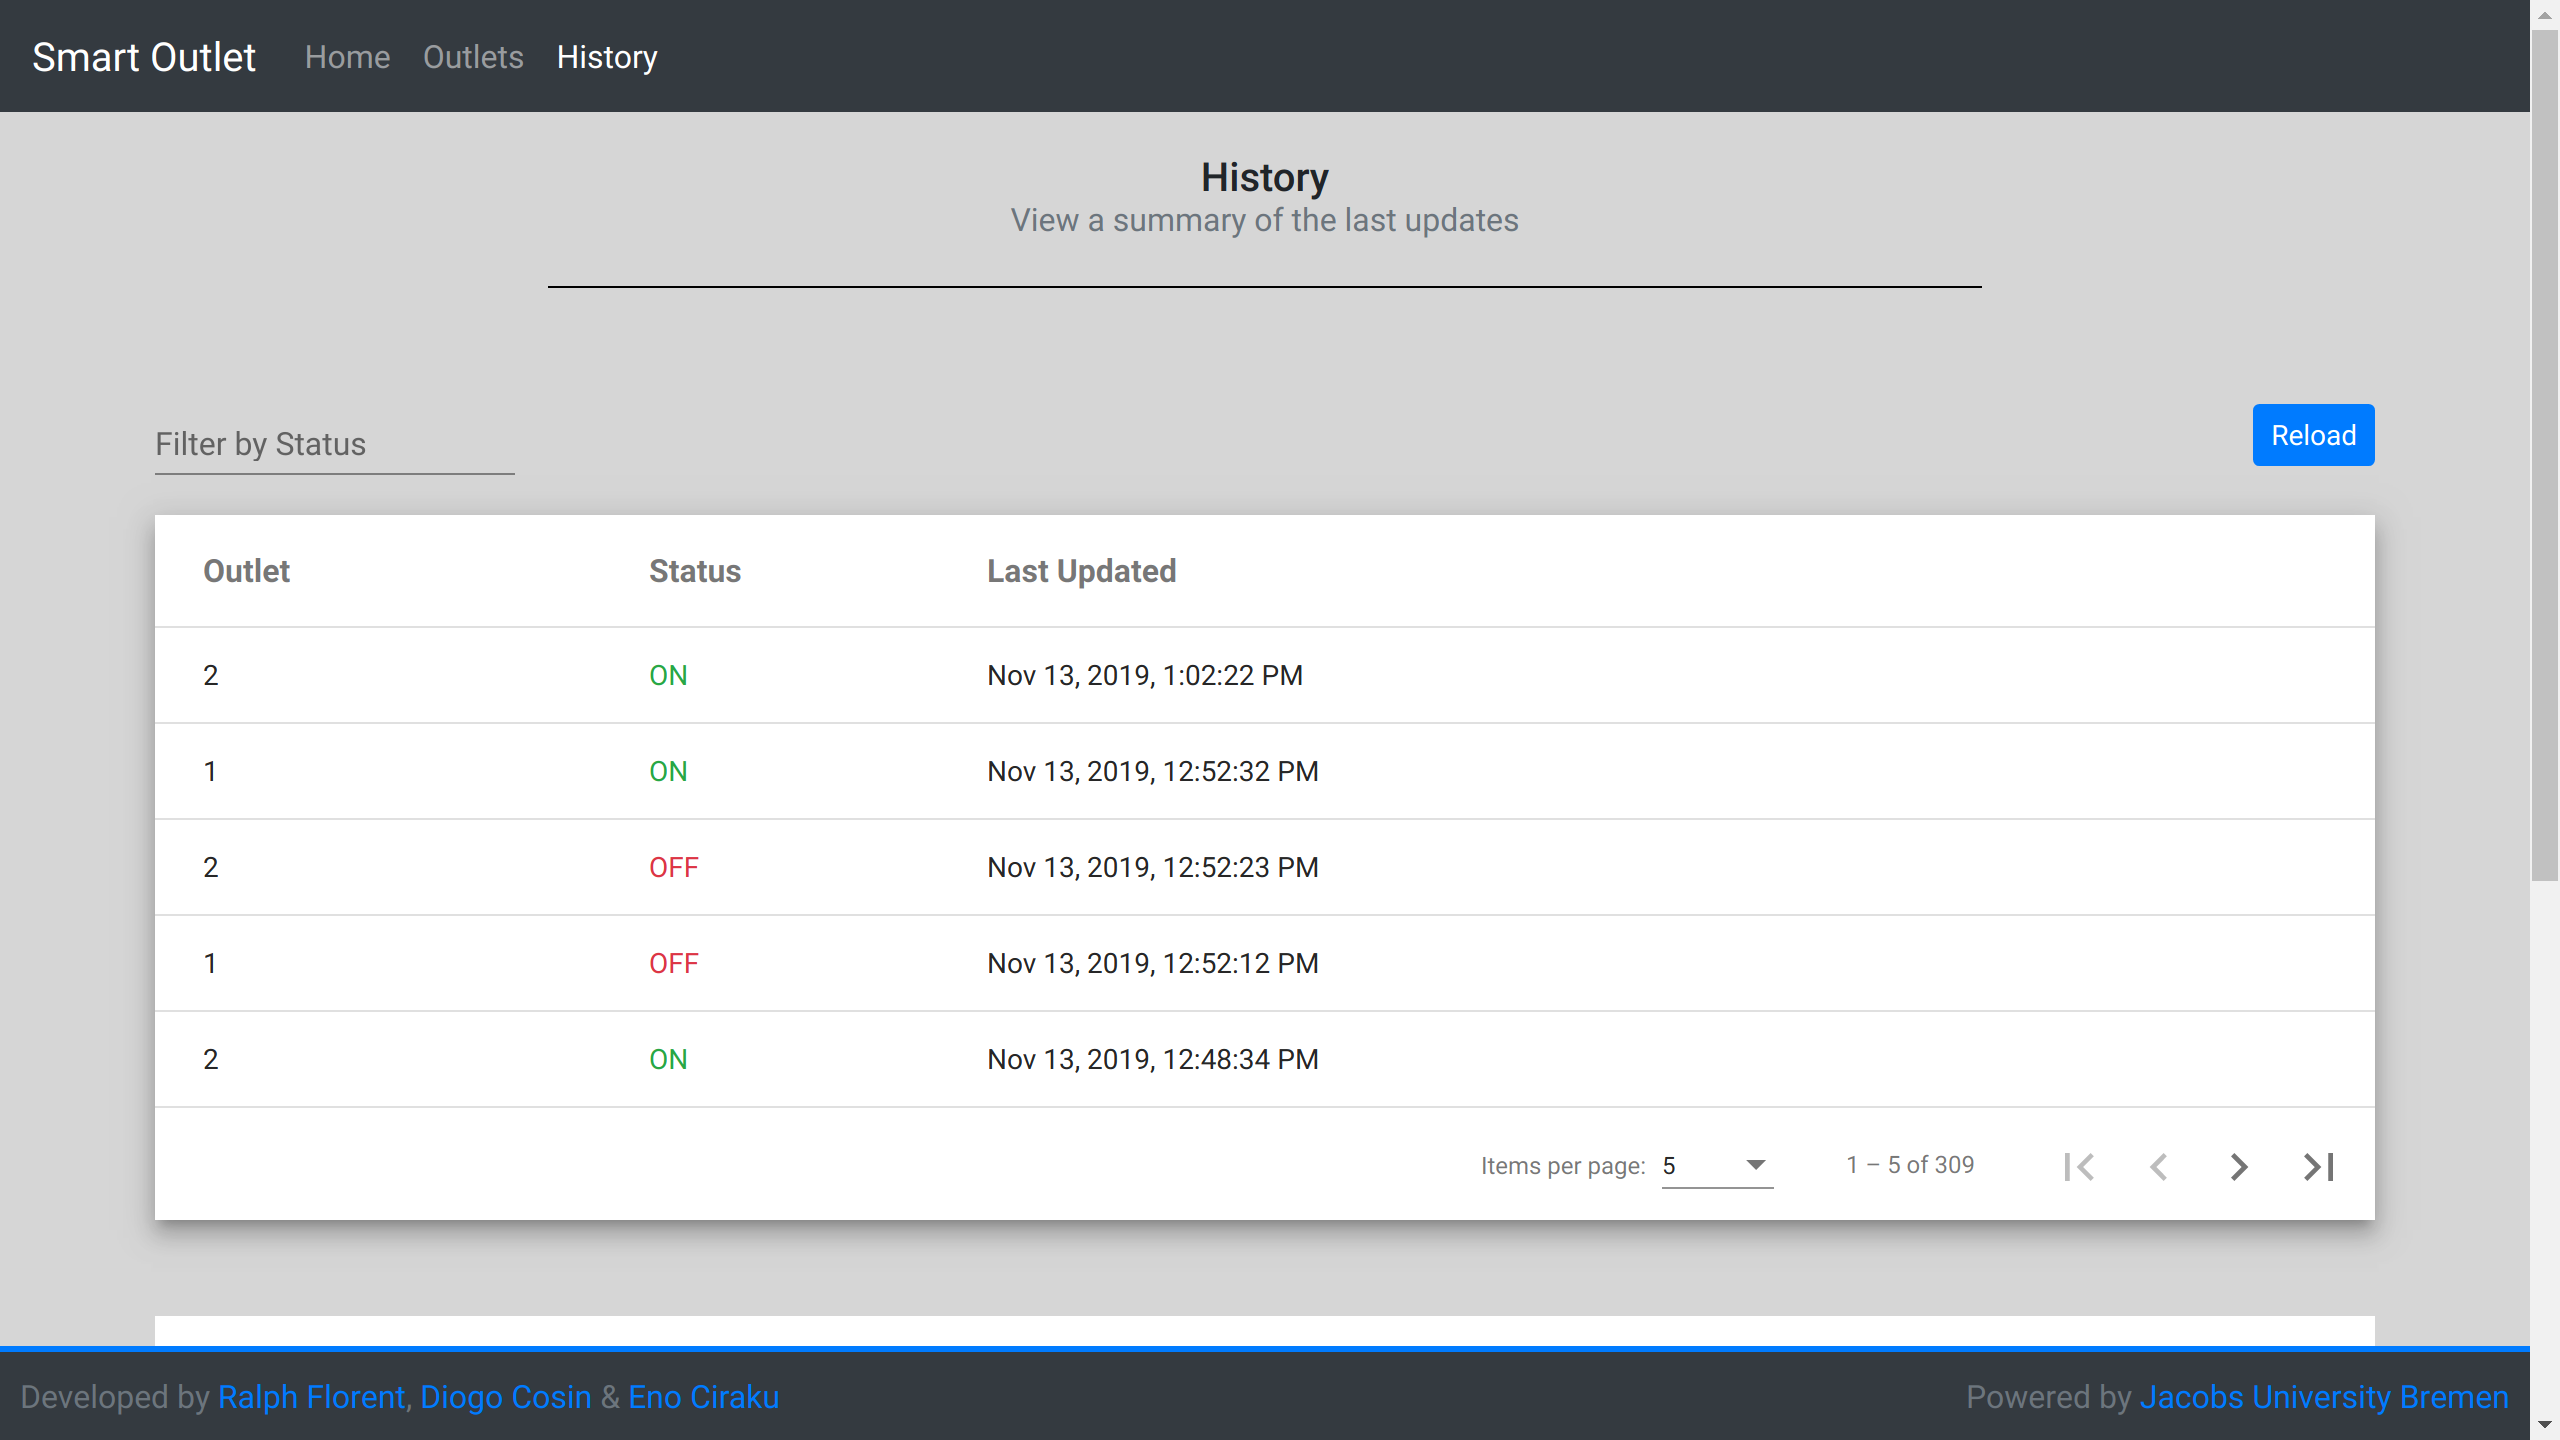
\includegraphics[scale=0.15]{screenshots/web-app/history.png}
    \caption{View of the history page}
    \label{fig:ui-history}
\end{figure}

\begin{figure}[ht!]
    \centering
    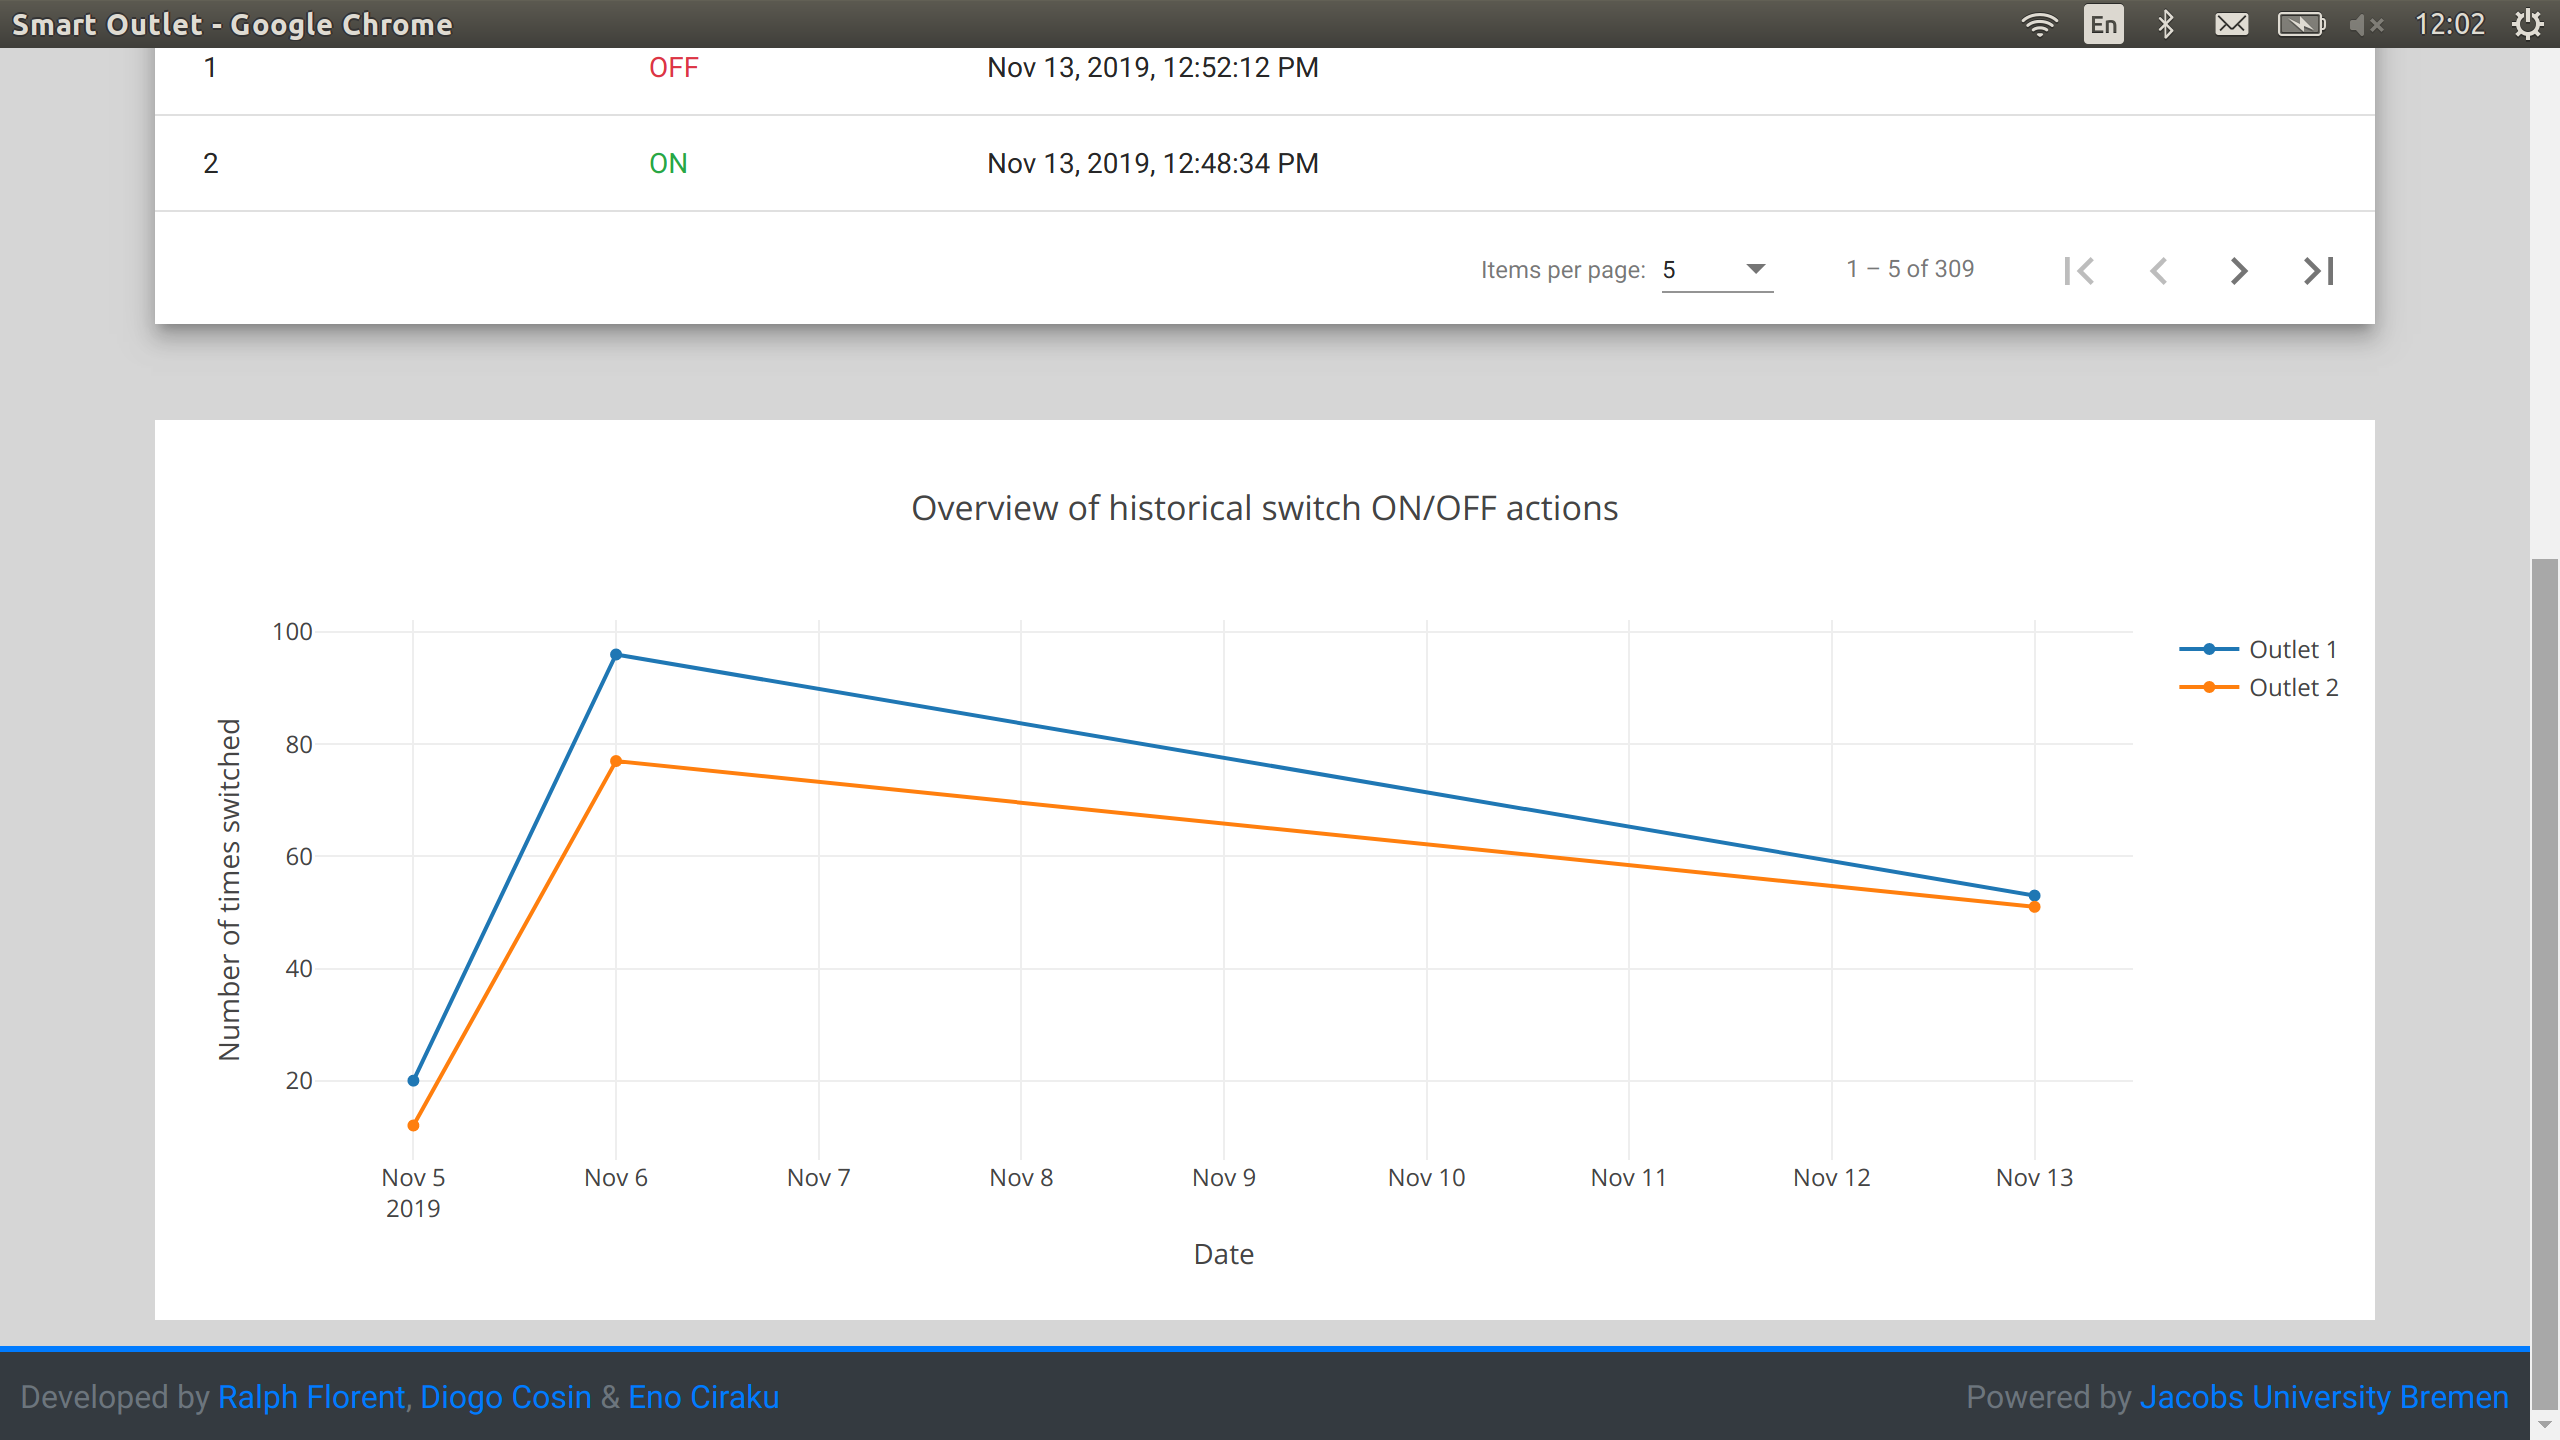
\includegraphics[scale=0.15]{screenshots/web-app/plot.png}
    \caption{View of the plot page}
    \label{fig:ui-plot}
\end{figure}

We do not detail much about the algorithm and data structure used for the web application since the main focus is not on how to build a web page efficiently. However, any curious developer is welcome to check the \textit{README} content of the web page to learn more about how to take a web app from development to production. Be aware that the programming techniques are well advanced and robust.

In addition to that, the web app is unit-tested and dockerized.
% ==============================================================================
% END: Methodology
% ==============================================================================

% Results and Discussions
\section{Results and Discussions}
\label{sec:res-and-disc}

% ==============================================================================
% END: Main Content
% ==============================================================================

% References
\clearpage
\newpage
\printbibliography

% Appendices
\clearpage
% Project - Technical Documentation
%
% Data Acquisition Technologies and Sensor Networks
% Jacobs University Bremen
% Supervisor: Prof. Dr. Fangning Hu
%
% Created on November 13, 2019
%
% Authors:
%   Ralph Florent <r.florent@jacobs-university.de>
%   Diogo Cosin <d.ayresdeoliveira@jacobs-university.de>
%   Eno Ciraku <e.ciraku@jacobs-university.de>
%
% Appendices part of the documentation

% ==============================================================================
% START: Appendix
% ==============================================================================

\clearpage
\appendix
\begin{appendices}
    \section{Code Repository}
    \label{sec:code-repo}

    All the code implemented during the execution of the prototype described in this report is available on the GitHub repository \href{https://github.com/ralflorent/smart-outlet}{https://github.com/ralflorent/smart-outlet}.

\end{appendices}
% ==============================================================================
% END: Scripts
% ==============================================================================

\end{document}
% ==============================================================================
% END: Scripts
% ==============================================================================